\documentclass[12pt,a4paper]{article}
\usepackage[utf8]{inputenc}
\usepackage[russian]{babel}
\usepackage[OT1]{fontenc}
\usepackage{amsmath}
\usepackage{amsfonts}
\usepackage{amssymb}
\usepackage{graphicx}
\usepackage[left=2cm,right=2cm,top=2cm,bottom=2cm]{geometry}
\title{\textbf{Лабораторная работа №5}\vspace{3mm} \\ 10.4 Магнитные моменты лёгких ядер}
\author{Петрушенко Валерия, 5111 гр.}
\date{Выполнено 24.10.2017}
\begin{document}
\maketitle
\renewcommand{\abstractname}{\vspace{-\baselineskip}}

\begin{abstract}
	В работе вычисляются магнитные моменты протона, дейтрона и ядра фтора на основе измерения их $g-$факторов методом ядерного магнитного резонанса (ЯМР). Полученные данные сравниваются с вычислениями магнитных моментов на основе кварковой модели адронов и одночастичной оболочеченой модели  ядер.
	
\end{abstract}

\section{Теория}

Отношение $\gamma$ магнитного момента к механическому называется гиромагнитным отношением:
\begin{equation}
\vec{\mu} = \gamma \vec{M}.
\end{equation}
Зачастую, вместо $\gamma$ используют более простую величину - $g$-фактор. Он также является отношением магнитного момента к механическому, но при этом магнитный момент измеряется в ядерных магнетонах Бора ($\mu_\text{я} = e \hbar / 2 m_p c$), а механический момент -- в единицах $\hbar$:
\begin{equation}
g = \frac{\mu / \mu _\text{я}}{M/\hbar} = \frac{\mu}{\mu_\text{я}} \frac{\hbar}{M} = \frac{\hbar}{\mu_\text{я}} \gamma.
\end{equation}
Отсюда 
\begin{equation} \label{mu}
\vec{\mu} = \frac{\mu_\text{я}}{\hbar} g \vec{M}.
\end{equation}


Проецируя $M$ и $\mu$ на направление вектора $B$, получаем:
\begin{equation}
\vec{\mu_B} = \frac{\mu_\text{я}}{\hbar} g \vec{M_B} = \mu_\text{я} g m.
\end{equation}
Наибольшее значение $\mu_B$ равно $\mu_\text{я} g I$. Его принято называть магнитным моментом ядра. 

Расстояние между двумя соседними компонентами расщепившегося в магнитном поле уровня:
\begin{equation} \label{deltaE}
\Delta E = B \Delta \mu_B = B \mu_\text{я} g \Delta m = B \mu_\text{я} g.
\end{equation}
~
Между компонентами расщепившегося уровня могут происходить электромагнитные переходы. Энергия квантов при этом определяется выражением (\ref{deltaE}), и явление носит резонансный характер. Частота излучения:

\begin{equation} \label{nu}
\nu = \frac{\Delta E}{h} = \frac{B \mu_\text{я} g}{h}.
\end{equation}

Возбуждение переходов между компонентами расщепившегося ядерного уровня - ядерный магнитный резонанс (ЯМР). 


~
В данной работе $g$-фактор определяется с помощью явления ЯМР. Изменяя частоту переменного магнитного поля, мы можем найти положение максимума поглощения, т.е. частоту резонанса. По этому максимуму определяется $g$-фактор из соотношения (\ref{nu}).

\section{Экспериментальная установка}

\begin{figure}[ht!]
 \centering
 {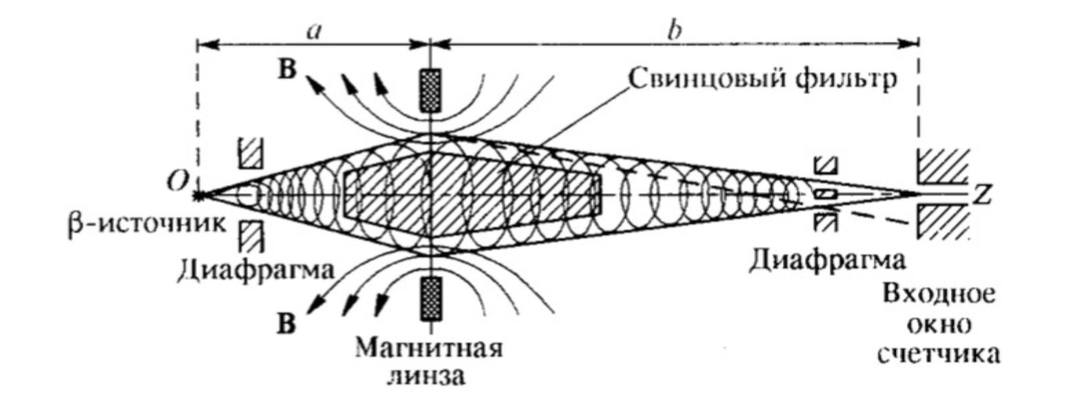
\includegraphics[width=0.6\linewidth]{scheme.png}}
\caption{Схема установки: 1 - часть индикаторной установки, исследуемый образец,3 - трансформатор,4 - электромагнит, 5 - катушки, 6 - модулирующие катушки, 8 - потенциометр }
\end{figure}


\section{Ход работы и обработка результатов}

Помещая разные образцы между полюсами электромагнита и устанавливая частоту $f_0$ индикаторной установки в диапазоне $1\div20$ МГц, плавно меняли магнитное поле в зазоре электромагнита, пока не обнаруживали сигнал ЯМР.

Полученные данные приведены в таблице:

\begin{table} [h]
	\centering
	\caption{Полученные данные для разных образцов}
	\begin{tabular}{|l||c|c|c|c|}
		\hline
		Образец № & 1 & 2 & 3 & 5 \\
		\hline
		$f$, МГц & 9,85 & 9,99 & 9,68 & 3,4 \\
		\hline
		$B$, мТл & 231 & 243 & 227 & 520 \\
		\hline
	\end{tabular}
\end{table}

По полученным данным определили $g-$факторы исследуемых ядер по формуле:

\begin{equation}
g_\text{я} = \frac{\hbar \omega_0}{\mu_\text{я} B_0} = \frac{h f_0}{\mu_\text{я} B_0}
\end{equation}

 Учитывая, что угловой момент протона определяется только его спином, рассчитали магнитный момент протона по формуле:
 
 	\begin{equation}
 	\mu = g_\text{я} \mu_\text{я}I
 	\end{equation}
 
 Предполагая, что  угловой момент внешнего протона в ядре фтора определяется только его собственным моментом (спином), рассчитали магнитный момент ядра фтора. 
 
 Рассчитанные данные свели в таблицу:


\begin{table} [h]
	\centering
	\caption{Обработанные данные} 
\begin{tabular}{|l||c|c|c|c|c|}
	\hline
Образец & $I$ & $g_\text{я}$ & $g_\text{я, табл.}$ & $\mu$ $(\text{в} ~\mu_\text{я})$ & $ \mu_\text{табл.}, \mu_\text{я} $ \\
\hline
1. Протон (резина)  & 0,5 & 5,601 & 5,58 & 2,8 & 2,79  \\
\hline
2. Ядро фтора   & 0,5 & 5,401 & 5,26 & 2,7 & 2,63  \\
\hline
3. Протон (вода)& 0,5 & 5,603 & 5,58 & 2,801 & 2,79  \\
\hline
5. Дейтрон  & 1 & 0,860 & 0,86 & 0,86 & 0,86  \\ 
\hline
\end{tabular}
\end{table}

\section{Вывод}
Вычислили магнитные моменты протона, дейтрона и ядра фтора, измерив их $g-$факторы методом ЯМР. Полученные данные оказались близки к табличным.



\end{document}